\documentclass[12pt]{article}
\usepackage[a4paper, margin=.30in]{geometry}
\usepackage{graphicx ,
            wrapfig,
            xcolor, 
            enumerate,
            amsmath,fontenc, mhchem,makecell, mhchem,tcolorbox
            }

\newcommand\headerMe[2]{\noindent{}#1\hfill#2}
\renewcommand{\thesection}{\Roman{section}}

\author{Zakaria HAOUZAN}
\date{\today}

\begin{document}
% headers --------------
\headerMe{Matière : Physique-Chimie}{Professeur : Zakaria HAOUZAN}\\
\headerMe{Unité : Transformations non totales d'un\\système chimique  }{Établissement : Lycée SKHOR qualifiant}\\
\headerMe{Niveau : 2BAC-SM-PC}{Heure : 6H}\\

% ------Content ________


%\begin{tabular}{|c|c|c|c|c|c|}
    %\hline
    %\multicolumn{2}{|c|}{Equation de la réaction}& \multicolumn{4}{c|}{
%\ce{CH_3COOH + H_2O <=>[1][2] CH_3COO^- + H_3O^+}}\\\hline
    %états  & avancement& \multicolumn{4}{|c|}{quantité de Matière en mol}\\\hline
	%Etat initial          &    0        &  $n_i$ &  - &  0              &  0 \\\hline
                 %\makecell{Etat de \\transformation}&    $x$      & $n_i -x$ & - & $x$  & $x$ \\\hline
				 %Etat final            & $x_{eq}$ & $n_i - x_{eq}$ & -  & $x_{eq}$&$x_{eq}$ \\\hline
   %% \cline{2-4}\
%\end{tabular}




\begin{center}

    \Large{Leçon $N^{\circ} 3.3 $: \color{red} Transformations associées à des réactions acido-basiques en solution aqueuse. }
\end{center}

\section{Le Produit ionique de l'eau : }
\subsection{Autoprotolyse de l'eau: } 
\subsubsection{Conductivité de l'eau:} 

l'eau pure est un mauvais conducteur du courant électrique et que son pH à $25^{\circ}C$ est $pH=7$.

\begin{itemize}
	\item La mauvaise conductivité de l'eau  est due à l'existence des ions oxoniums $H_3O^+$
		et des ions hydroxydes $HO^-$ qui résultent de l'autoprotolyse de l'eau dont l'équation s'écrit: 

		\ce{H_2O_{(l)} + H_2O_{(l)} <=>[1][2] H_3O^+_{(aq)} + HO^-_{(aq)}}
	\item Cette réaction dans le sens (1) s'appelle la réaction d'autoprotolyse de l'eau.
	\item Le $pH$ de l'eau pure à $25^{\circ}C$ est : $pH=7$ donc l'eau pure est électriquement neutre : 

		$[H_3O^+] $=$[HO^-]$=$10^{-7}mol/L$ Considérons 1L d'eau pure à $25^{\circ}C$ ,de pH=7.

\end{itemize}

Tableau d'avancement : 
\begin{center}
\begin{tabular}{|c|c|c|c|c|}
	\hline
	\multicolumn{2}{|c|}{Equation de la réaction}& \multicolumn{3}{c|}{
	\ce{2H_2O_{(l)} <=>[1][2] H_3O^+ + HO^-}}\\\hline
	états  & avancement& \multicolumn{3}{|c|}{quantité de Matière en mol}\\\hline
	Etat initial &0&  $n_i$ &  0&  0 \\\hline
\makecell{Etat de \\transformation}&$x$ & $n_i -x$ & $x$  & $x$ \\\hline
				 Etat final            & $x_{eq}$ & $n_i - x_{eq}$ & $x_{eq}$&$x_{eq}$ \\\hline
   % \cline{2-4}\
\end{tabular}
\end{center}


la quantité de Matière initiale de l'eau : $n_i$ =$\frac{m}{M} = \frac{\rho_{eau}.V}{M} = \frac{1g/cm^3 . 10^3.cm^3}{18} = 55,5mol$

On a $[H_3O^+]$ = $10^{-pH}$ = $\frac{x_{eq}}{V}$ 

donc $x_{eq}$ = $10^{-pH}.V = 10^{-7}.1L = 10^{-7} mol$

Pour L'avancement maximal correspond à la disparition totale de l'eau, ($x_{max} = \frac{n_i}{2}$)

Le taux d'avancement à l'équilibre $\tau = \frac{x_{eq}}{x_{max}} = 3,6.10^{-7} \%$

Donc l'autoprotolyse de l'eau est une réaction très limitée.


\subsection{Produit ionique de l'eau . }
La réaction d'autoprotolyse de l'eau se produit dans toutes les solutions aqueuses.
La constante d'équilibre associée à la réaction d'autoprotolyse de l'eau est :$$K_e = [H_3O^+]_{(eq)}.[HO^-]_{(eq)}$$

Ke : s'appelle le produit ionique de l'eau.(il ne dépend que de la température).

On utilise aussi le pKe qui est lié au produit ionique par la relation suivante:
$K_e = 10^{-pKe}$ et $pKe$=$-log(Ke)$.


Dans toutes les solutions aqueuses à $25^{\circ}C$ : $K_e = [H_3O^+].[HO^-]=10^{-14}$ donc $pKe = 14$

\begin{center}
	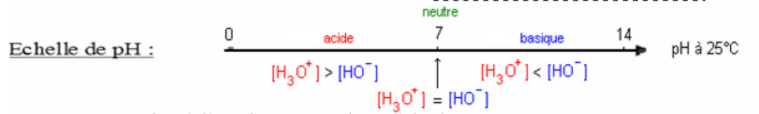
\includegraphics[width=0.7\textwidth]{./img/echellePH.png}
\end{center}

\section{Constante d'acidité d'un couple acide-base : }

\subsection{Définition : }
Pour un couple acide -base A/B , la réaction de l'acide A avec l'eau s'écrit: \ce{A + H_2O <=> B + H_3O^+}

La constante d'acidité du couple acide-base A/B s'écrit: $K_A = \frac{[B][H_3O^+]}{[A]}$

C'est une gradeur sans unité, qui ne dépend que de la température.

On utilise aussi le pKA qui est lié à la constante d'acidité par la relation suivante:
$K_A =  10^{-pKA}$ et $pKA = -log(K_A)$

\subsection{Relation entre le pH et pKA: }
D'après la relation de la constante d'acidité on a:$K_A = \frac{[B][H_3O^+]}{[A]}$ donc $[H_3O^+] = \frac{[A]K_A}{[B]} $

aussi $pH = -log([H_3O^+])$ et $pH = -log(K_A) - log(\frac{[A]}{[B]})$

alors $$pH = pKA + log(\frac{[B]}{[A]})$$


\subsection{La constante d'équilibre K associée à une réaction acido-basique : }

Pour le couple acide/base $A_1/B_1$ : \ce{A_1 + H_2O <=> B_1 + H_3O^+} la constante d'acidité $K_{A1}$=$\frac{[B_1][H_3O^+]}{[A_1]}$
\\Pour le couple acide/base $A_2/B_2$ : \ce{A_2 + H_2O <=> B_2 + H_3O^+} la constante d'acidité $K_{A2}$=$\frac{[B_2][H_3O^+]}{[A_2]}$

Dans la réaction acido-basique entre l'acide A1 du couple A1/B1 et la base B2 du couple A2/B2:

\ce{A_1 + B_2 <=> A_2 + B_1} la constante d’équilibre $$K=\frac{[A_2][B_1]}{[A_1][B_2]} = \frac{K_{A1}}{K_{A2}} = 10^{pKA1 - pKA2}$$


\section{Comparaison du comportement des acides et des bases : }
\subsection{Comparaison des forces des acides : }
\subsubsection{Influence du taux d'avancement final sur la force de l'acide : }
Un acide $A_1H$ est plus fort qu'un acide $A_2H$, si, \underline{à concentrations égales}, le taux d'avancement de sa réaction avec l'eau
est plus grand que celui de la réaction de l'acide $A_2H$ avec l'eau. $\tau_1\geq \tau_2 $).
\\Pour des solutions de mêmes concentrations, l’acide le plus fort est celui dont le taux d’avancement final est le plus élevé.
donc c’est celui pour lequel $[H_3O^+]$ est la plus élevée.

$[H_3O^+]$ et $pH$ varient en sens inverses $(pH=-log[H_3O^+])$. 

donc: l’acide le plus fort est celui pour lequel le pH est le plus faible

\subsubsection{Influence de la constante d'acidité:}

Tableau d'avancement de la réaction d'un acide A de concentration c , avec l'eau (volume de la solution V).:


\begin{tabular}{|c|c|c|c|c|c|}
	\hline
	\multicolumn{2}{|c|}{Equation de la réaction}& \multicolumn{4}{c|}{
\ce{A + H_2O <=>[1][2] B + H_3O^+}}\\\hline
	états  & avancement& \multicolumn{4}{|c|}{quantité de Matière en mol}\\\hline
	Etat initial          &    0        &  $n_i=C.V$ &  - &  0              &  0 \\\hline
				 \makecell{Etat de \\transformation}&    $x$      & $C.V -x$ & - & $x$  & $x$ \\\hline
				 Etat final            & $x_{eq}$ & $C.V - x_{eq}$ & -  & $x_{eq}$&$x_{eq}$ \\\hline
   % \cline{2-4}\
\end{tabular}

L'eau est utilisée en excès, donc l'acide A est le réactif limitant. et Taux d'avancement à l'équilibre : $\tau = \frac{x_{eq}}{C.V}$.
\\Avec $[H_3O^+] = [B] = \frac{x_{eq}}{V} = \frac{\tau.C.V}{V} = \tau.C$ et $[A] = \frac{C.V - X_{eq}}{V} = C(1-\tau)$
\\La constante: d'acidité: $$K_A = \frac{[B][H_3O^+]}{[A]} = \frac{(C.\tau)^2}{C(1-\tau)} = \frac{C\tau^2}{1-\tau}$$

\textbf{Un acide est d’autant plus fort que sa constante d’acidité KA est plus grande ou que son pKA est plus petit.}



\subsection{Comparaison des forces des bases: }
\subsubsection{Influence du taux d'avancement final sur la force de la base: }
Une base B1 est plus forte qu’une base B2 ,si, à concentrations égales, le taux d’avancement de sa réaction avec l’eau
est plus grand que celui de la réaction de la base B2 avec l’eau. ( $\tau_1>\tau_2$.)


\subsubsection{Influence de la constante d'acidité: }
Tableau d'avancement de la réaction de la base B de concentration c avec l'eau(volume de la solution V) .:


\begin{tabular}{|c|c|c|c|c|c|}
	\hline
	\multicolumn{2}{|c|}{Equation de la réaction}& \multicolumn{4}{c|}{
\ce{B + H_2O <=>[1][2] A + HO^-}}\\\hline
	états  & avancement& \multicolumn{4}{|c|}{quantité de Matière en mol}\\\hline
	Etat initial          &    0        &  $n_i=C.V$ &  - &  0              &  0 \\\hline
				 \makecell{Etat de \\transformation}&    $x$      & $C.V -x$ & - & $x$  & $x$ \\\hline
				 Etat final            & $x_{eq}$ & $C.V - x_{eq}$ & -  & $x_{eq}$&$x_{eq}$ \\\hline
   % \cline{2-4}\
\end{tabular}

L'eau est utilisée en excès, donc La base B est le réactif limitant. et Taux d'avancement à l'équilibre : $\tau = \frac{x_{eq}}{C.V}$

On a  $[B] = \frac{C.V-x_{eq}}{V} = C(1-\tau)$ et $[HO^-] = [A] = \frac{x_{eq}}{V} = C\tau$

la constante d’équilibre associée à cette réaction : $$K = \frac{[A].[HO^-]}{[B]} = \frac{(C\tau)^2}{C(1-\tau)} = \frac{C\tau^2}{1-\tau}$$


D'autre parte on a :	$K_A = \frac{[B].[H_3O^+]}{[A]} = \frac{Ke}{K} = \frac{1-\tau}{C.\tau}.Ke$


\textbf{Une base est d’autant plus forte que la constante d’acidité KA associée au couple acide/base auquel elle appartient est plus petite
ou que le pKA correspondant est plus grand.}

\section{Diagramme de prédominance et celui de distribution : }

\subsection{Diagramme de prédominance : }

Relation liant le pH et le pKA est: $pH = pK_A + log(\frac{[B]}{[A]})$
\\Si pH = pKA ; $log(\frac{[B]}{[A]}) = 0 $ donc $\frac{[B]}{[A]} = 1$ [B] = [A] acune des espèces A et B ne prédomine  
\\Si $pH > pKA$ ; $log(\frac{[B]}{[A]}) > 0 $ donc $\frac{[B]}{[A]} > 1$ alors $[B] > [A]$ la base B prédomine  
\\Si $pH < pKA$ ; $log(\frac{[B]}{[A]}) < 0 $ donc $\frac{[B]}{[A]} < 1$ alors $[B] < [A]$ l'acide A prédomine  

Diagramme de prédominance:

\begin{center}
	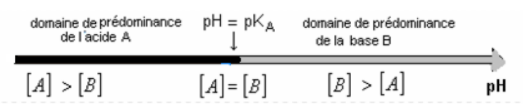
\includegraphics[width=0.5\textwidth]{./img/domainonace.png}
\end{center}



\subsection{Diagramme de répartition : }

On considère une solution contenant l'acide A et sa base conjuguée B.
\\On appelle pourcentage de l'acide A dans la solution, $\alpha(A) = \frac{[A]}{[A]+[B]}$
\\On appelle pourcentage de la base B dans la solution, $\alpha(B) = \frac{[B]}{[A]+[B]}$
\\Des logiciels de simulation permettent de donner les courbes représentant les pourcentages des espèces acide A et
basique B d’un même couple dans une solution en fonction du pH de cette solution. On donne l’allure générale de
cette distribution :.


\begin{center}
	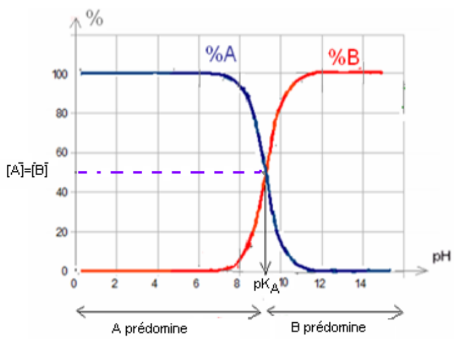
\includegraphics[width=0.5\textwidth]{./img/dominPH.png}
\end{center}

\subsection{Les Indicateur colorés : }
Un indicateur coloré est un couple acide base $HIn/In^-$ ,dont les la forme acide HIn et la forme basique Inont des teintes différentes en solution aqueuse.
\\Pour le bleu de bromothymol par exemple: la couleur de HIn est jaune et celle de $In^-$ est bleue.

La forme acide HIn de l'indicateur réagit avec l'eau : \ce{HIn + H_2O <=> In^- + H_3O^+}


Donc le pH de la solution est lié au pKA de l'indicateur coloré par la relation suivante :$pH = pKA + log({\frac{[In^-]}{[HIn]}})$


\begin{itemize}
	\item Lorsque la valeur du pH est voisine de celle du pKA , les deux formes HIn et Insont présentes avec des concentrations
voisines , il y'a superposition des deux teintes et la couleur observée est dite teinte sensible.

\item Généralement l'une des teintes prédomine et impose sa couleur si sa quantité est k fois supérieure à celle de l'autre.

\item  la valeur de k dépend de l'indicateur , pour le (BBT) k=9 , c'est-à-dire si la concentration de HIn qui est jaune est 9 fois
supérieure à celle de Inqui est bleu il prédomine et sa teinte apparait ) ceci qui entraine l'existence d'un intervalle de pH qui
correspond à la teinte sensible qu'on appelle : la zone de virage.
On donne dans le tableau suivant la zone de virage de quelques indicateurs colorés
\end{itemize}

\begin{center}
	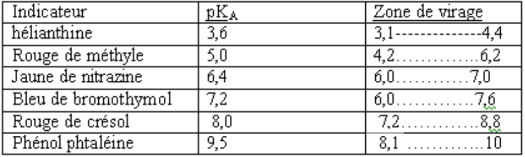
\includegraphics[width=0.5\textwidth]{./img/table.png}
\end{center}



%\begin{figure}[h!]
	%\begin{center}
	%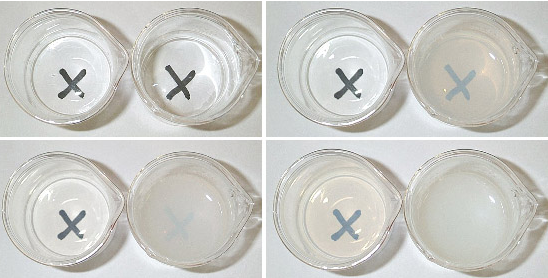
\includegraphics[width=0.5\textwidth]{./img/TRLconcentration.png}
%\end{center}
%\vspace{-1cm}
%\end{figure}



%\begin{wrapfigure}[10]{r}{0.5\textwidth}
%    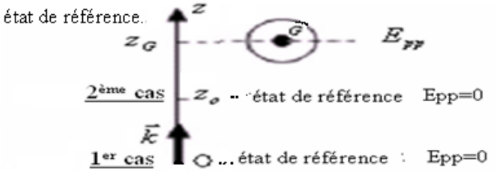
\includegraphics[width=0.5\textwidth]{./img/img00.png}
%\end{wrapfigure}


%\begin{center}
   %\begin{tabular}{|c|c|c|}
      %\hline
      %Indicateur coloré & Couleur de l’espèce acide & Couleur de l’espèce base\\\hline
      %BBT               & Jaune                     & Bleue\\\hline
      %Hélianthine       &Rose                       & Jaune\\\hline
      %Phénolphtaléine   & inclore                   & rose \\\hline
   %\end{tabular}
%\end{center}

\end{document}

